\subsection{Problem Statement}\label{ps}

Most of the algorithms for robotic table tennis need to specify when, where and how to intercept the incoming ball trajectory $\ball(t)$. In \citet{Matsushima05} and \citet{Muelling11} for example, the authors calculate the intersection point of a predicted ball trajectory $\ballPred(t)$ with a virtual hitting plane (VHP) at $y = y_{\mathrm{VHP}}$ to determine the space and time coordinates of the hitting event. Although additional constraints like the VHP can simplify trajectory generation, they can also lead to awkward or infeasible movements. It is possible to eliminate this plane altogether and include the striking time as another parameter to be determined in an optimization problem.

%
%\subsection{Optimal Control for Trajectory Generation}
%
When generating striking trajectories for a robot with $n$ degrees of freedom, trajectories with minimal acceleration can be preferred for safety and efficiency reasons. Consider the following \emph{free-time} optimal control problem~\citep{Liberzon11}
%
\begin{align}
\min_{\ddot{\joint},T} & \int\limits_{0}^{T} \ddot{\joint}(t)^{\mathrm{T}}\vec{R}\ddot{\joint}(t) \ \mathrm{d}t \label{costFnc1} \\
\text{s.t. }  
&\hitFun\big(\joint(\hitTime),\hitTime\big) \in \hit, \label{hitFunc} \\
&\netFun\big(\joint(\hitTime),\dot{\joint}(\hitTime),\hitTime\big) \in \net, \label{netFunc} \\
&\landFun\big(\joint(\hitTime),\dot{\joint}(\hitTime),\hitTime\big) \in \landEvent, \label{landFunc} \\
& \joint(0) = \joint_{0}, \label{initCond1} \\
& \dot{\joint}(0) = \dot{\joint}_{0}, \label{initCond2}
\end{align}
%
\noindent where the final hitting time $\hitTime$ is an additional variable to be optimized along with the joint accelerations $\ddot{\joint}(t) \colon [0,\hitTime] \to \mathbb{R}^{n}$. The weighting matrix $\vec{R}$ for the accelerations is positive definite. %i.e., $\vec{R} \succ 0 \in \mathbb{R}^{n \times n}$. 
Initial conditions for the robot are the joint positions $\joint_0$ and joint velocities $\dot{\joint}_0$.
%$\vec{T}(\cdot) \in \mathbb{R}^{4 \times 4}$ 
The inequality constraints \mbox{\eqref{hitFunc} -- \eqref{landFunc}} ensure that the task requirements for table tennis are satisfied. The hitting constraint $\hitFun \in \hit$ ensures impact of the racket with the ball at striking time $T$. The net constraint $\netFun \in \net$ makes sure the ball passes over the net and finally, the landing constraint $\landFun \in \landEvent$ captures the requirement that the ball should bounce first on the opponents court. See Figure~\ref{tableTennisConstraints} for an illustration. The precise definitions of these constraint functions and the constraint sets will be introduced in section~\ref{method2}.
% These algorithms can possibly lead to different play styles, depending on the higher level strategy.

Solutions of \mbox{\eqref{costFnc1} -- \eqref{initCond2}} can be found using Pontryagin's minimum principle~\citep{Pontryagin}. The optimal $\joint(t)$ in both cases is a third degree polynomial for each degree of freedom, with the inequality constraints \mbox{\eqref{hitFunc} -- \eqref{landFunc}} imposing generalized \emph{transversality conditions} on the Hamiltonian and the momenta to satisfy at striking time~\citep{BrysonHo69,Schaettler12}. Solving such boundary value problems is hard, especially given real time constraints. In the later sections we will introduce two algorithms that will solve this problem efficiently under additional constraints. These two approaches can be seen as different ways to solve the underlying table tennis task efficiently and they lead to two different play-styles. 

%See Figure~\ref{mainIdea} for an illustration.

When given only constraints at the boundary, the striking time $T$, the joint position and velocity values at striking time $\joint_f$ and $\dot{\joint}_f$ fully parametrize this problem. The polynomial coefficients for the striking trajectory
%
\begin{align}
\joint_{\mathrm{strike}}(t) = \vec{a}_3 t^3  + \vec{a}_2 t^2 + \dot{\joint}_0 t + \joint_0, 
\end{align} %\ 0 \leq t \leq T,
%
\noindent can then be determined in joint-space for each degree of freedom of the robot
%can be parameterized in terms of final joint positions $\joint_f$, final joint velocities $\dot{\joint}_f$ and striking time $T$
%
\begin{gather}
\begin{aligned}
\vec{a}_3 &= \frac{2}{T^3}(\joint_0 - \joint_f) + \frac{1}{T^2}(\dot{\joint}_0 + \dot{\joint}_f), \\
\vec{a}_2 &= \frac{3}{T^2}(\joint_f - \joint_0) - \frac{1}{T}(\dot{\joint}_f + 2\dot{\joint}_0).
\label{coeffs}
\end{aligned}
\end{gather}
%
% After computing the parameters $T, \joint_f, \dot{\joint}_f$, we generate also a returning trajectory $\joint_{\mathrm{return}}(t)$ to the same initial posture $\joint_0$ with an appropriately chosen return time $\returnTime$. The return time can be chosen sufficiently long to guarantee feasibility of the returning trajectory. 

The notation that is used frequently in the rest of the paper is shown in Table~\ref{tableSymbols} for the reader's convenience.
%Initially the robot will not be moving, $\dot{\joint}_0 = 0$.
%
\begin{figure}
	\centering
	\includegraphics[width=0.5\textwidth]{tableTennisConstraints.pdf}%
	\caption{In table tennis, robot trajectories (blue) can be seen as reactions to predicted ball trajectories (orange). The players are free to decide where, when and how to intercept the ball. However, the resulting outgoing ball trajectories need to be \emph{feasible}: the ball has to pass above the net and land on the opponent's court. The feasible region above the net is drawn in transparent green. The rules of the game can be captured as constraints for generating robot striking trajectories.}
	\label{tableTennisConstraints}
\end{figure}
%
%
\begin{figure*}
	\centering
	\def\svgwidth{2.0\columnwidth}
	\input{Figures/predictionModels.pdf_tex}
	%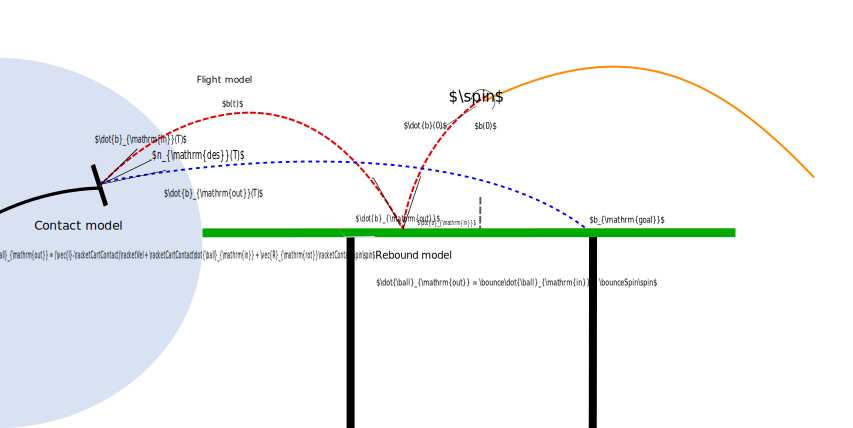
\includegraphics[width=0.8\textwidth]{predictionModels.pdf}%
	\caption{Ball prediction schema for table tennis. After estimating the initial ball position, velocity and spin, the future path of the ball can be predicted using the flight model, the rebound model and the racket-ball contact model. The trajectory generation framework uses these models to compute desired striking trajectories.}
	\label{tableTennisSchema}
\end{figure*}
%
%
\begin{table}[b!]
	\small\sf\centering
	%\renewcommand{\arraystretch}{1.3}
	\caption{Table of Symbols}
	\label{tableSymbols}
	\resizebox{\columnwidth}{!}{%
	\begin{tabular}{c|l}
		%\hline
		\toprule
		\bfseries Notation & \bfseries Explanation \\ %	{\small \bfseries Notation}
		\midrule
		%\hline
		$\hitTime$ & hitting time \\
		$\restTime$ & return time \\
		$\landTime$ & desired ball landing time after hit \\
		%$\predTime$ & prediction horizon for incoming ball \\
		$\ballLand$ & desired ball landing positions \\
		$\joint(t)$ & joint trajectory \\
		$\ballPred(t)$ & predicted ball trajectory \\
		$\racket(t)$ & racket center position \\
		$\racketVel(t)$ & racket velocity \\
		$\normal(t)$ & racket normal \\
		$\kin_p$ & kinematics function for racket center position \\ 
		$\kin_n$ & kinematics function for racket normal \\
		$\jac(\joint_f)$ & jacobian at hitting time \\                 
		$\normal_{\mathrm{des}}(T)$ & desired racket normal at hitting time \\
		$\racketVel_{\mathrm{des}}(T)$ & desired racket velocity at hitting time \\
		$\spin$ & ball spin \\
		$\dot{\ball}_{\mathrm{in}}, \dot{\ball}_{\mathrm{out}}$ & ball velocity before and after impact \\
		$\numBallsMin$ & minimum number of balls to start prediction \\
		$\joint_0, \dot{\joint}_0$ & initial joint positions and velocities \\
		$\joint_{\mathrm{cur}}, \dot{\joint}_{\mathrm{cur}}$ & joint position and velocity estimates \\
		$\joint_f, \dot{\joint}_f$ & joint position and velocity at hitting time \\
		$\joint_{\mathrm{ext}}$ & joint extreme values of trajectory \\
		$\jointMax, \jointMin$ & joint angle upper and lower limits \\
		$\vec{R}$ & weighting matrix \\
		$\joint_{\mathrm{strike}}(t)$ & joint striking trajectory \\
		$\joint_{\mathrm{return}}(t)$ & joint returning trajectory \\
		$\hitFun,\landFun, \netFun$ & table tennis task constraints \\
		%$\joint_{\mathrm{des}}$ & strike \& return trajectory \\
		%$\vec{\tau}$ & torques computed by inverse dynamics \\
		%\bottomrule
	\end{tabular}
}
\end{table}
%
\subsection{Background on Ball Prediction}\label{sectionPredict} % Predicting with Ball Models
 
For the trajectory generation process, three ball models will be used to determine the table tennis task constraints \mbox{\eqref{hitFunc} -- \eqref{landFunc}}: ball flight model, ball-table rebound model and ball-racket contact model. Whenever an incoming ball is detected in midair, a flight model will first be used to predict the trajectory $\ballPred(t)$ of the ball centre of mass coordinates $\ball = (b_x,b_y,b_z)^{\mathrm{T}}$ until impact with a racket, table or ground. 

\paragraph{Flight model.} Table tennis balls are very light, a standard ball weighs about $2.7$ grams, which makes nonlinear effects due to air drag and spin noticeable especially when the ball speed $\ballVel = \|\dot{\ball}\|_2$ is high. The \emph{flight model}~\citep{Nakashima10}
%
\begin{align}
%\big(\ddot{b}_x, \ddot{b}_y, \ddot{b}_z\big)^{\intercal} = \big(-\drag \ballVel \dot{b}_x, -\drag \ballVel \dot{b}_y, \gravity - \drag \ballVel \dot{b}_z\big)^{\intercal} \label{flightModel}
\ddot{\ballPred} = \gravityVec -\drag\ballVel \, \dot{\ballPred} + \lift \spin \times \dot{\ballPred}, \label{flightModel}
\end{align}
%
\noindent is a nonlinear dynamics model that incorporates air drag and spin effects. The air drag constant $\drag$ and the lift constant $\lift$ as well as gravity $\gravity$, $\gravityVec = (0,0,\gravity)^{\mathrm{T}}$, parameterize this model. The \emph{magnus effect} due to spin (angular velocity) $\spin$, for example, acts as an additional downward force for an incoming ball if the angular velocities are in the negative $x$-direction (topspin). It is assumed that spin stays constant throughout the ball motion.
%
\paragraph{Rebound Model.} Formally, rebound is a discrete event which reflects the ball velocity when the ball hits the table. The incoming velocities  $\dot{\ball}_{\mathrm{in}}$ at bouncing time are transformed to outgoing velocities $\dot{\ball}_{\mathrm{out}}$. The following nonlinear \emph{rebound model}~\citep{Nakashima10} for a standard ball with radius $\ballRadius = 2$ cm,
%
\begin{align}
\dot{\ball}_{\mathrm{out}} = \bounce\dot{\ball}_{\mathrm{in}} + \bounceSpin\spin,
\label{reboundModel}
\end{align}
%
\noindent is parameterized by the dynamic coefficient of friction $\coeffFrictionTable$ and the coefficient of restitution $\coeffRestitutionTable$ of the table
%
\begin{align}
\scalemath{0.9}{\bounce} &= \scalemath{0.8}{\begin{bmatrix}
1 - \alpha & 0 & 0 \\
0 & 1 - \alpha & 0 \\
0 & 0 & -\coeffRestitutionTable
\end{bmatrix}} , \
\scalemath{0.9}{\bounceSpin} = \scalemath{0.8}{\begin{bmatrix}
0 & \alpha\ballRadius & 0 \\
-\alpha\ballRadius & 0 & 0 \\
0 & 0 & 0
\end{bmatrix}},
\end{align}
%
\noindent where the nonlinearity comes from the term
%
\begin{align}
\alpha &= \coeffFrictionTable(1 + \coeffRestitutionTable)\tfrac{\dot{b_z}}{\|\dot{\ball}_T\|},
\end{align}
%
\noindent $\dot{\ball}_T$ is the \emph{tangent velocity} at contact
%
\begin{align}
\dot{\ball}_T &= (\dot{b}_x - \ballRadius \omega_y, \dot{b}_y + \ballRadius \omega_x, 0)^{\mathrm{T}},
\end{align}
%
\noindent for $\spin = (\omega_x, \omega_y, \omega_z)^{\mathrm{T}}$. This model suggests, for example, that some amount of topspin is transferred at sliding impact to linear velocity in the y-direction. See Figure~\ref{tableTennisSchema} for a table tennis schema. 

\paragraph{Racket Contact Model.}  We assume the following linear racket contact model holds for a standard racket with radius $\racketRadius \approx 7.6$ cm,
%
\begin{align}
\vec{o} = \racketContact\vec{i} + \racketContactSpin\spin,
\label{contactModel}
\end{align}
%
\noindent between the outgoing ball velocity $\vec{o}$ and the incoming ball velocity $\vec{i}$, similar to~\eqref{reboundModel} but in the moving racket frame. The outgoing ball Cartesian velocities are hence found by multiplying $\vec{o}$ with the racket rotation matrix and adding the racket velocities, i.e., $\dot{\ball}_{\mathrm{out}}(t) = \vec{R}_{\mathrm{rot}}\vec{o}(t) + \racketVel(t)$, where the rotation matrix $\vec{R}_{\mathrm{rot}}(\joint(t))$ of the racket is given by the kinematics function. The impact model is parameterized by the constants $\kappa$ and $\coeffRestitutionRacket$
%
\begin{align}
\scalemath{0.8}{\racketContact} &= \scalemath{0.8}{\begin{bmatrix}
1 - \kappa & 0 & 0 \\
0 & 1 - \kappa & 0 \\
0 & 0 & -\coeffRestitutionRacket
\end{bmatrix}}, \ 
\scalemath{0.8}{\racketContactSpin} = \scalemath{0.8}{\begin{bmatrix}
0 & \kappa\racketRadius & 0 \\
-\kappa\racketRadius & 0 & 0 \\
0 & 0 & 0
\end{bmatrix}}.
\label{racketMatrices}
\end{align}
%
Letting $\racketCartContact := \vec{R}_{\mathrm{rot}}\racketContact\vec{R}_{\mathrm{rot}}^{\mathrm{T}}$, we get the following relationship between the Cartesian velocities:
%
\begin{align}
\dot{\ball}_{\mathrm{out}} = (\vec{I}-\racketCartContact)\racketVel + \racketCartContact\dot{\ball}_{\mathrm{in}} + \vec{R}_{\mathrm{rot}}\racketContactSpin\spin.
\end{align}

%
%racket velocity $\racketVel$ and racket normal $\normal$. Equation~\eqref{contactModel} is a generalization of the \emph{mirror law}~\cite{Muelling11}, where the outgoing velocity of the ball as a result of contact is calculated as a simple reflection %The matrix $\contactModel \in \mathbb{R}^{3 \times 9}$
%%
%\begin{align}
%o_{n} - v_{n} = -\epsilon_{R} (i_{n} - v_{n}),
%\label{mirrorLaw}
%\end{align}
%%
%\noindent with $v_{n}$ the speed of the racket along its normal $\normal(t)$ and $\epsilon_{R} \in [0,1]$ the coefficient of restitution of the racket. Scalars $o_{n}$ and $i_{n}$ are the outgoing and incoming ball speeds along the racket normal, respectively. This model \eqref{mirrorLaw} assumes an elastic momentum exchange and in our experience, it is quite inaccurate, especially at high ball velocities, as will be shown empirically in section~\ref{results}.

\paragraph{Ball Prediction.} The models~\mbox{\eqref{flightModel} -- \eqref{racketMatrices}} can be composed together to predict the future ball trajectory given camera observations. We use an Extended Kalman Filter (EKF) to estimate the ball state from observations~\citep{Sorenson85}. The ball state for the filter is the ball positions and velocities, since we assume that the ball spin is constant throughout motion. The ball spin can be seen as a parameter of the prediction functions. 
% Any other regression method to estimate initial ball position and velocity can also be used. 

EKF instantiated with the models~\eqref{flightModel} -- \eqref{racketMatrices}, the initial ball positions $\ball_0$ and velocities $\dot{\ball}_0$ and spin $\spin$, estimates the evolving ball state and predicts the future ball trajectory at each time instant $t$: a multivariate normal distribution $p_t(\ball,\dot{\ball})$ of ball states parameterized by time is generated
%
\begin{align}
\big(\ball(t)^{\intercal},\dot{\ball}(t)^{\intercal}\big)^{\intercal} &\sim p_t(\ball,\dot{\ball}) = \mathcal{N}(\vec{\mu}(t),\vec{\Sigma}(t)),
%\label{ballProcess}
\end{align}
%
\noindent where $\vec{\mu}(t) = \big(\ballPred(t)^{\intercal},\dot{\vec{b}}(t)^{\intercal}\big)^{\intercal}$ is the mean ball position and velocity predictions. The covariance matrix $\vec{\Sigma}(t)$ is updated along with the mean estimate $\vec{\mu}(t)$ using the EKF predict and update equations. The covariance matrices are used to reject outliers and hence make Kalman Filtering more robust to ball detection errors.
%This typically happens when the vision system~\citep{Lampert12} cannot reliably detect a flying orange ball in the image.
% among other things
